\documentclass[conference]{IEEEtran}
\usepackage{cite}
\usepackage{amsmath}
\usepackage{amsfonts}
\usepackage{amssymb}
\usepackage{xcolor}
\definecolor{light-gray}{gray}{0.95}
\definecolor{airforceblue}{rgb}{0.36, 0.54, 0.66}
\definecolor{amber}{rgb}{1.0, 0.75, 0.0}
\usepackage[skins]{tcolorbox}
\usepackage{setspace}
\tcbset{commonstyle/.style={boxrule=0pt,sharp corners,enhanced jigsaw,nobeforeafter,
	boxsep=0pt,left=\fboxsep,right=\fboxsep}}
\newtcolorbox{mycolorbox}[1][]{commonstyle,#1}
\usepackage{array}
\usepackage{color}
\usepackage{colortbl}

%--------package image---------------------------------------------------------
\usepackage{graphicx}
\usepackage{subfig}
\graphicspath{{./imgs/}}
\renewcommand{\figurename}{Fig.}

%-------package tikz-----------------------------------------------------------
\usepackage{tikz,fp,ifthen,fullpage}
\usepackage{pgfmath}
\usetikzlibrary{backgrounds}
\usetikzlibrary{decorations.pathmorphing,backgrounds,fit,calc,through,
decorations.markings}
\usetikzlibrary{arrows}
\usetikzlibrary{shapes,decorations,shadows}
\usetikzlibrary{fadings}
\usetikzlibrary{patterns}
\usetikzlibrary{mindmap}
\usetikzlibrary{decorations.text}
\usetikzlibrary{decorations.shapes}
\usepackage{pgfplots}
\pgfplotsset{compat=1.13}
%--------------------------Document--------------------------------------------
\begin{document}
%Here goes the title
	\title{Rapid development of a neural network for image classification using 
	fine-tuning techniques and implementation on SoC systems}
%Authors List
	\author
	{\IEEEauthorblockN{Francesco Argentieri}
		\IEEEauthorblockA{ID 183892\\
		Email: francesco.argentieri@studenti.unitn.it}
		%\and
		%\IEEEauthorblockN{Author 2}
		%\IEEEauthorblockA{University\\
		%Location\\
		%Email: }
	}
	\maketitle
%Main body
	% abstract
	\begin{abstract}
The intent of this project is the rapid development of a neural network for
image classification. 
After a brief theoretical presentation of the functioning of a neural network,
the reader is introduced to the world of deep neural networks and classification. 
Thanks to the use of framework like Keras is possible to develop refinement 
techniques starting from already known models.
There is discussion of the architecture of a USB commercial device, Intel 
Movidius neural compute stick, with low power consumption for neural network 
execution on SoC systems such as Raspberry.
Finally, there are the problems and limitations that occurred during the 
development and distribution of the software implemented.
\end{abstract}
% define keyword
	\begin {IEEEkeywords}
		Python, Keras, Movidius, Intel, Neural Network, Inception, TensorFlow, 
		ImageNet, ncsdk, API, backend.
	\end{IEEEkeywords}
	%Introduction
	\section{Introduction}
\label{sec:intro}
In this era, a large amount of structured and unstructured data became available.
\textbf{Machine Learning} (\textbf{ML}) has evolved as a branch of artificial
intelligence: it envisages the development of self-learning algorithms, which are
capable of acquiring knowledge from data with the aim of making predictions.
Instead of requiring a human presence who manually enact the rules and
build models for the analysis of large amounts of data, machine learning offers
a more efficient alternative to capture the knowledge in the data. Machine learning
aims to gradually improve the performance of forecasting models and
to make data driven decisions.
In this section we will examine the three different types of machine learning:
\emph{supervised learning}, \emph{unsupervised learning} and
\emph{reinforcement learning}.
Where we will show the fundamental differences between these types of
learning.\cite{raschka2016machine}
%
\subsection{Supervised learning}
\label{subsec:supervised-learnig}
The main purpose of supervised learning is to derive a model from 
training data, which allows us to make predictions for data that are not
available or future.
Here, the term ``supervision" refers to the fact that the output signal labels 
of the sample sets are already known.
A supervised learning task, which is based on discrete class labels, is also 
called a classification task, in figure \ref{fig:supervised-learning-scheme} it 
is possible to observe a process diagram.
Another supervised learning subcategory is regression, whose resulting
signal is a continuous value.
Classification is a sub-category of supervised learning, which has the goal to
provide class category labels for new instances, based on observations made in
the past.
These labels are discrete, unordered values ​​that can be considered as
belonging to a group of instances.
However, the set of class labels does not necessarily have to be a binary
nature.
The predictive model identified by a supervised learning algorithm can consider
each class label that is present in the learning dataset of a new instance, which
is not labelled.\\
A typical example of \emph{multi-class classification} is the recognition of
hand-written text.\cite{raschka2016machine}
%
\begin{figure}[!h]
\centering
%\draw [help lines] (0,0) grid (8,8);
\resizebox{\linewidth}{!}{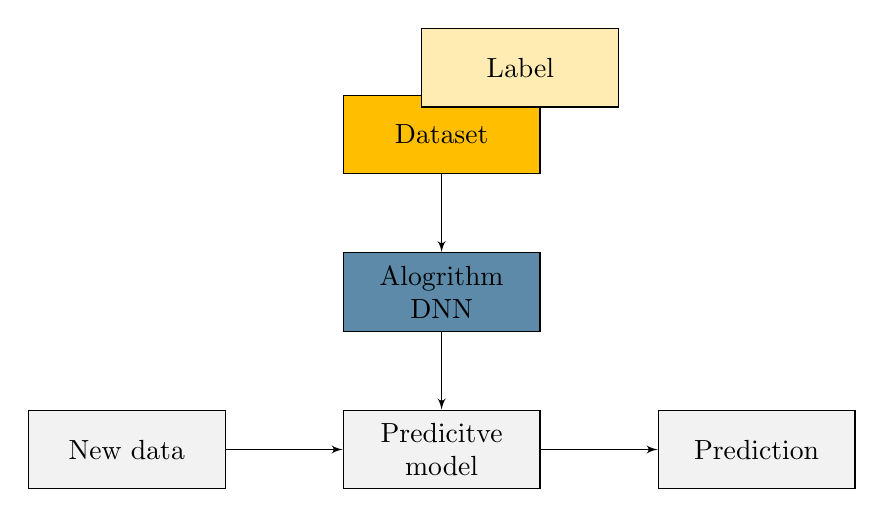
\begin{tikzpicture}[auto,>=latex']
%\draw [help lines] (0,0) grid (8,8);
\tikzset{
	boxA/.style={
  		rectangle,
  		inner sep=0pt,
  		text width=25mm,
  		align=center,
  		draw=black,
  		fill=airforceblue,
  		minimum height = 10mm
  	},
  	boxB/.style={
  		rectangle,
  		inner sep=0pt,
  		text width=25mm,
  		align=center,
  		draw=black,
  		fill=amber,
  		minimum height = 10mm
  	},
  	boxB1/.style={
  		rectangle,
  		inner sep=0pt,
  		text width=25mm,
  		align=center,
  		draw=black,
  		fill=amber!30,
  		minimum height = 10mm
  	},
  	boxC/.style={
  		rectangle,
  		inner sep=0pt,
  		text width=25mm,
  		align=center,
  		draw=black,
  		fill=light-gray,
  		minimum height = 10mm
  	},
  }

\node (a) [boxC, align=center] at (1,1) {New data};
\node (b) [boxC, align=center] at (5,1) {Predicitve\\ model};
\node (c) [boxC, align=center] at (9,1) {Prediction};
\node (d) [boxA, align=center] at (5,3) {Alogrithm\\ DNN};
\node (e) [boxB, align=center] at (5,5) {Dataset};
\node (e1) [boxB1, align=center] at (6,5.85) {Label};
\draw [->] (a) -- (b);
\draw [->] (b) -- (c);
\draw [->] (d) -- (b); 
\draw [->] (e) -- (d); 
\end{tikzpicture}}
\caption{supervised learning scheme} 
\label{fig:supervised-learning-scheme}
\end{figure}
%
\subsection{Reinforcement learnig}
\label{subsec:reinforcement-learnig}
Another type of machine learning is reinforcement learning.
Here, the goal is to develop a system (\emph{agent}) for people to improve
their performance. In order to do so, that system is based on interactions with 
the environment.
Since information relating to the current state of the environment
include also a \emph{reward} signal, we can consider strengthening
learning as an example of supervised learning.
However, this feedback is not the correct label or the
true value of truth, but it represents the quality of the measurement of the 
performance measured by the reward function.
Through interaction with the environment, an agent can then use reinforcement
learning to learn a series of actions, which maximize this reward through a
trial-and-error exploratory approach or deliberative planning.\cite{raschka2016machine}
%
\begin{figure}[!h]
\centering
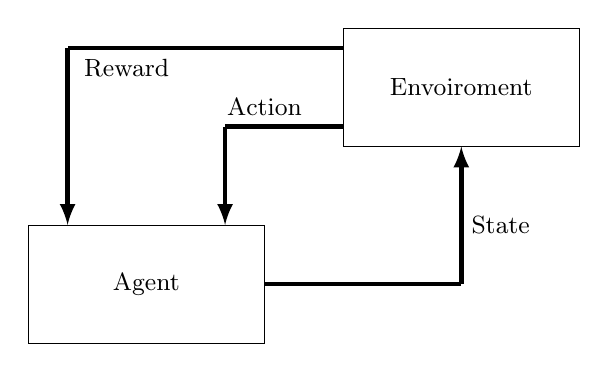
\begin{tikzpicture}[>=latex]
 %\draw [help lines] (0,0) grid [step=0.5] (8,4);
 \draw (0.5,0) rectangle ++(3cm, 1.5cm);
 \draw (4.5,2.5) rectangle ++(3cm,1.5cm);
 %\node [draw] (1.5,2) {Agent};
 \coordinate [label={[font=\small]center:Agent}] (A) at (2,0.75);
 \coordinate [label={[font=\small]center:Envoiroment}] (E) at (6,3.25);
 \draw [-, ultra thick] (3.5,0.75) -- (6,0.75);
 \draw [->, ultra thick] (6,.75) -- (6,2.5);
 \coordinate [label={[font=\small]center:State}] (S) at (6.5,1.5);
 %
 \draw [-, ultra thick] (4.5,2.75) -- (3,2.75);
 \draw [->, ultra thick] (3,2.75) -- (3,1.5);
 \coordinate [label={[font=\small]center:Action}] (T) at (3.5,3);
 %
 \draw [-, ultra thick] (4.5,3.75) -- (1,3.75);
 \draw [->, ultra thick] (1,3.75) -- (1,1.5);
 \coordinate [label={[font=\small]center:Reward}] (R) at (1.75,3.5);
\end{tikzpicture} 
\caption{reinforcement learning scheme} 
\label{fig:reinforcement-learning-scheme}
\end{figure}
%
\subsection{Unsupervised learning}
\label{subsec:unsupervised-learning}
In supervised learning, we know in advance the correct answer when we describe
our model, while in reinforcement learning we define a measure, or reward, for
the specific actions performed by the agent.
In unsupervised learning, on the other hand, we are dealing with unlabelled data
or data from the unknown structure.
Using unsupervised learning techniques, we are able to observe the structure of
our data, to extract meaningful information from them without being able to
rely on the guide nor a variable known relative result, nor a reward function.
Clustering is an exploratory technique of data analysis that allows us to
organize a series of information within meaningful groups (\emph{cluster})
without having any previous knowledge of memberships in such groups.
Each cluster that can be derived during the analysis defines a group of objects
that share a certain degree of similarity, but which are more dissimilar than
the objects present in the other clusters, which is why clustering is sometimes
called \emph{``unsupervised classification"}.
Clustering is an excellent technique for structuring information to identify
meaningful relationships in the data.\cite{raschka2016machine}
%
\begin{figure}[!h]
\centering
\includegraphics[width=\linewidth]{cluster}
\caption{example of clustering}
\label{fig:unsupervised-learning-scheme}
\end{figure}
%
%\subsection{Prerequisites}
%\label{subsec:rerequisites}
%The code requires Python 3.5.2 or higher (version 3.7 is not supported) to be
%installed on a MacOS, Linux or Windows system.
%Referring to essential libraries dedicated to the scientific group, including
%SciPy, NumPy, scikit-learn, matplolib and pandas.
%We will add the TensorFlow-gpu library for efficient training of neuronal
%networks on GPU units.

	\section{Deep learning}
\label{sec:deeplearning}
%
Deep learning lies at the heart of the most advanced machine learning solutions,
such as those that have learned to recognize items and images, determine the
sentiment of text, and drive vehicles. 
These neural networks are complex and can be challenging to build, but Keras 
removes much of the effort.
Keras acts as an API\footnote{An Application Programming Interface (API) 
provides an abstraction for a problem and specifies how clients should interact 
with the software components that implement a solution to that
problem.\cite{api}}, 
letting us quickly create a network that might take hours or days to hand code 
in Python or other languages.
%
\subsection{Introducing Keras}
\label{subsec:introduction_keras}
Let's use the definition from the documentation at keras.io.
Keras is a high-level neural network API, written in Python and capable of
running on top of \emph{TensorFlow}, \emph{CNTK} or 
\emph{Theano}\cite{chollet2015keras, tensorflow2015-whitepaper}.
That is, it lets us build neural networks easier by providing us with a
high-level set of constructs.
These constructs handle much of the plumbing involving in wring up neural
networks and thus reduce programming errors.
Also, as an API, it provides an interface that we can develop against and a
detailed description of what happens when we invoke various objects and methods.
Keras is Python centric in its code and is implemented as a Python library.
It is imported and used just like any other Python library you might be familiar
with, so the learning curve is minimal.
Finally, Keras runs on top of \emph{TensorFlow}, \emph{CNTK}, or \emph{Theano}.
These are three of the most widely used libraries for performing work with
neural networks.
Keras calls these libraries to perform the actual execution of operations that
create, populate, train, and evaluate the neural networks we specify in Keras.
Keras utilizes either TensorFlow, CNTK, or Theano as the 
\emph{backend}\footnote{In software engineering, the terms front end and back 
end refer to the separation of concerns between the presentation layer (front 
end), and the data access layer (back end) of a piece of software, or the 
physical infrastructure or hardware. In the client--server model, the client 
is usually considered the front end and the server is usually considered the 
back end, even when some presentation work is actually done on the server.
\cite{backend}}.
Keras itself does not create or execute the neural network.
Rather, Keras defines an API we code against. 
In our code we invoke Keras methods and pass the appropriate parameters.
Keras evaluates these for correctness and constructs whatever objects are
required.
Keras then calls the appropriate backend methods to do the actual neural 
network operations, such as defining structures, training the neural network 
model, and evaluating the trained model. Any result from these operations are 
returned by the backend to Keras, which processes them and returns to our code 
the appropriate results.
%
\begin{figure}[!h]
\centering
\includegraphics[width=\linewidth]{enviroment}
\caption{Block diagram environment}
\label{fig:kerasenvoiroment}
\end{figure}
%
\section{Neural Networks}
\label{sec:neuralnetwork}
%
The neural network, in figure \ref{fig:nn_layer}, that can be divided into trhee
parts, takes data from input nodes and feeds the network.
This data could be values from a data table, images from a camera, sounds from a
recording, or output from a sensor.
The input layer does not change the data, it simply passes it for processing by
the remaining layers. The data from the input layer is passed to another layer
of neurons.
These layers can be of different types with the different layer types performing
different transformations on the data as required by our solution. In a simple
network, the input layer can be directly connected to an output layer of neurons,
which provide the final outputs.\linebreak
%
\begin{figure}[!h]
\centering
\includegraphics[width=\linewidth]{neuralnetwork}
\caption{Neural networks layers}
\label{fig:nn_layer}
\end{figure}
%
\\But in most networks, the input layer is connected to hidden layers.
Hidden layers are defined as not being input or output layers, and therefore,
are hidden to the code that's using the neural network.
The network can have many hidden layers and if there are two or more hidden
layers we call the network a deep neural network, as shows in figure 
\ref{fig:deepnn}.
%
\begin{figure}[!h]
\centering
\includegraphics[width=\linewidth]{deep_nn}
\caption{Deep neural networks layers}
\label{fig:deepnn}
\end{figure}
%
In this learning process we adjust the structures of our neurons.
To understand this, let's look at a single neuron. Here we see the inputs and
outputs we showed in the network diagram, with the inputs going in and the
outputs going out.
However, what is not showing in this diagram is how the neurons work internally.
To do that, we need to open the neuron so we can see how it is constructed.
As we see, the neuron is performing a simple mathematics summing of weights, 
times the input value and adds a bias.
The product of these operations is passed through a non-linear activation
function.
And the output of the activation function is the output of the neuron.
A key feature of the neural network is the ability to use the input data to
train the weights and biases so the signal passed out of the neuron changes
based on the input data. To do this training, we expose the network to data.
With each set of data, an algorithm is used to adjust the weights and bias to
minimize the error the network has in predicting the data's values.
This is done through processes called forward propagation and back propagation.
And when these processes are complete, the network is said to be trained, and
the weights and biases of all the neurons have been adjusted to give the best
results on the training data. So to summarize, the neural network consists of
three layer types: input, hidden, and output. 
By passing training data through the network, the network of neurons is 
trained to give results with the least error.
This training is done by adjusting weights and biases in the neurons, utilizing
the processes of forward propagation and back propagation, and if there are two
or more hidden layers in the network, we say it's a deep neural network.

	\section{Building Convolutional Neural Network with Keras}
\label{sec:buildcnn}
%
As we discussed in section (\ref{subsec:introduction_keras}), Keras 
has a series of layers that were specifically created to support convolutional 
neural networks.
By definition, a fully connected layer connects every neuron in the layer and 
at the first layer it's connected to all the inputs. 
And all these connections create a problem known as the curse of 
dimensionality. 
That is, the more neurons and connections we have, the more weights we must 
train. 
This issue appears often, it is one of reasons why deep neural networks can 
take a long time to learn. 
To understand this issue a bit more, let's consider the case of working with 
images. 
Assume that we have an 8 megapixel image and that we want to learn 
something from this image. 
To do that, we construct a network with a dense layer. 
Since every pixel in the image can contain unique data, they each contribute 
uniquely to determining the logic resulting from analysing the image. 
Therefore we need to connect each pixel to each neuron in our first layer. 
Let's say that we have 1000 neurons in the first dense layer.
We have to connect the data from each pixel to each neuron so we end up with 
1000 neurons connected to 8 million pixel values, with each connection having 
its own weight that needs to be trained. 
That works out to 8 billion weights we have to train. 
And with most images it's even more. In a color image, each pixel has three 
colors. 
One for red, green, and blue channels of the image. 
So there are actually 24 billion weights to train.
Solving this explosion in the number of weights we have to train is one of the 
key reasons convolutional neural networks were developed. 
%
\subsection{How works CNNs}
\label{ssec:cnnworks}
%
Convolutional neural network address our two concerns of working with image 
type data namely, many weights to train and being able to detect objects based 
on their general appearance rather than precisely matching an image. 
A lot of research has been performed when working with images and has 
resulted in subtle layers that you find in almost all convolutional neural 
networks. 
And these are the convolution layers you find in Keras. 
To understand the function of these layers, let's go over the structure of a 
convolutional neural network, which classifies objects and images.
%
Let's walk through this diagram so we can get an overview of how convolutional 
neural networks work and how we implement them using Keras. 
We see the image data is passed through the convolutional layer, then through 
a non-linear ReLU activation and then to a pool layer. 
And then to a second convolution with ReLU layer and a second pool layer. 
Finally, to a fully connected layer and then to a second fully connected 
layer for classification. 
So we can divide our convolutional neural network into four operations. 
Convolution, non-linearity, you see via ReLU, pooling, and classification. 
You will find these four operations in almost all convolutional neural networks. 
Let's look at each operation in detail so we understand how to set parameters 
and pass data when we construct our convolutional neural network in Keras.
Convolutional neural networks are the current state-of-art architecture for
image classification. They are used in practice today in facial recognition, self
driving cars, and detecting whether an object is a hot-dog.
%
\subsection{Convolution}
\label{ssec:convolution}
%
A convolution consists of a kernel, shows in figure \ref{fig:convolution}, 
(green square above), also called filter,
that is applied in a sliding window fashion to extract features from the input.
This filter is shifted after each operation across the input by an amount called
strides. At each operation, a matrix multiply of the kernel and current region
of input is calculated. Filters can be stacked to create high-dimensional
representations of the input.
%
\begin{figure}[!h]
\centering
\includegraphics[width=\linewidth]{conv_arithmetic}
\caption{Convolution operation to extract features from the input}
\label{fig:convolution}
\end{figure}
%
There are two ways of handling differing filter size and input size, namely
same padding and valid padding.
Same padding will pad the input border with zeros (as seen above) to ensure the
input width and height are preserved. Valid padding does not pad.
Typically, you will want to use same padding or you will rapidly reduce the
dimensionality of your input.
Finally, an activation function (typically a ReLU\footnote{In the context of 
artificial neural networks, the rectifier is an activation function defined as 
the positive part of its argument:\\ \(f(x) = x^{+} = \text{max}(0,x)\)}), 
represented in figure \ref{fig:relu}, is applied to give the convolution non-linearity.
ReLU’s are a bit different from other activation functions, such as sigmoid or
tanh, as ReLUs are one-sided.
This one-sided property allows the network to create sparse representation
(zero value for hidden units), increasing computational efficiency.
%
\begin{figure}[htb]
\centering
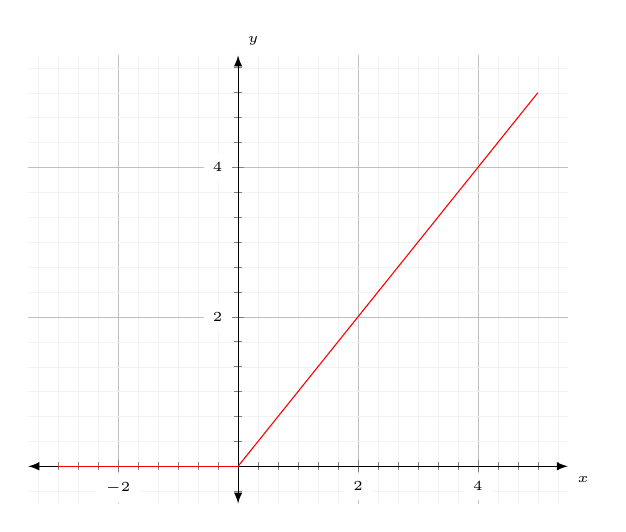
\begin{tikzpicture}
    \begin{axis}[
        domain=-3:5,
        grid=both,
    	grid style={line width=.1pt, draw=gray!10},
    	major grid style={line width=.2pt,draw=gray!50},
    	axis lines=middle,
    	minor tick num=5,
    	enlargelimits={abs=0.5},
    	axis line style={latex-latex},
    	ticklabel style={font=\tiny,fill=white},
    	xlabel style={at={(ticklabel* cs:1)},anchor=north west},
    	ylabel style={at={(ticklabel* cs:1)},anchor=south west},
    	xlabel={\tiny $x$},
    	ylabel={\tiny $y$}
    ]
        \addplot+[mark=none,red,domain=-3:0] {0};
        \addplot+[mark=none,red,domain=0:5] {x};
    \end{axis}
\end{tikzpicture}
\caption{Rectified linear unit (\textbf{ReLU})\\ \(F(x) = x^{+} = \text{max}(0,x)\)}
\label{fig:relu}
\end{figure}
%
\subsection{Pooling}
\label{ssec:pooling}
Pooling is an operation to reduce dimensionality. 
It applies a function summarizing neighbouring information.
Two common functions are max pooling and average pooling.
By calculating the max of an input region, the output summarizes intensity of
surrounding values.
Pooling layers also have a kernel and padding, and are moved in strides, as 
represented in figure \ref{fig:pooling}.
To calculate the output size of a pooling operation, you can use the formula:
\begin{equation}
 \text{Input Width} - \text{kernel width} + 2 * \text{padding}  / \text{strides} + 1
\end{equation}
%
\begin{figure}[htb]
\centering
\includegraphics[width=\linewidth]{pooling}
\caption{Max pooling is the application of a moving window across a 2D input 
space, where the maximum value within that window is the output}
\label{fig:pooling}
\end{figure}
%
\subsection{Fully Connected Layer}
\label{ssec:fully_connected}
Fully connected layers you are likely familiar with from neural networks.
Each neuron in the input is connected to each neuron in the output;
fully-connected.
Due to this connectivity, each neuron in the output will be used at most one
time.
%
\begin{equation}
  \sum_{i=1}^{n} \,  x \, \cdot \, W+b
\end{equation}
%
\begin{figure}[htb]
\centering
\includegraphics[width=\linewidth]{fully_connected}
\caption{Deep neural networks layers}
\label{fig:fully_connected}
\end{figure}
%
\\\noindent In a CNN, the input is fed from the pooling layer into the fully connected layer.
Depending on the task, a regression or classification algorithm can be applied
to create the desired output, a representative example is shown in figure \ref{fig:fully_connected}.

	\section{The project}
\label{sec:project}
The goal of this project is the rapid development of a neural network for low 
power systems, hence the need to resort to a technique known as 
'fine-tuning' for the realization of our neural network.
In general, if our dataset is not drastically different in context from the 
dataset which the pre-trained model is trained on, we should go for 
fine--tuning.
Pre-trained network on a large and diverse dataset like the \emph{ImageNet} 
captures  universal features like curves and edges in its early layers, that are
relevant and useful to most of the classification problems.
Of course, if your data set represents some very specific domain, we should 
then consider training the network from scratch.
One other concern is that if our dataset is small, fine-tuning the pre-trained 
network on a small dataset might lead to over-fitting, especially if the last few 
layers of the network are fully connected layers, as in the case for \emph{VGG} 
network. 
If we have a few thousand raw samples, with the common data augmentation 
strategies implemented (translation, rotation, flipping, etc.), fine-tuning will 
usually get us a better result.
%
\subsection{Fine-tuning Techniques}
\label{subsec:fine-tuning}
Some general guidelines for fine-tuning implementation:
\begin{itemize}
\item The common practice is to truncate the last layer (softmax layer) of the
pre--trained network and replace it with our new \emph{softmax} layer that are
relevant to our own problem. For example, pre-trained network on \emph{ImageNet} 
comes with a \emph{softmax} layer with $1000$ categories.
\end{itemize}
If our task is a classification on $10$ categories, the new \emph{softmax} layer
of the network will be of $10$ categories instead of $1000$ categories.
We then run back propagation on the network to fine-tune the pre--trained 
weights. Make sure cross validation is performed so that the network will be 
able to generalize well.
\begin{itemize}
\item  Use a smaller learning rate to train the network. 
Since we expect the pre--trained weights to be quite good already as compared 
to randomly initialized weights, we do not want to distort them too quickly and 
too much. 
A common practice is to make the initial learning rate $10$ times smaller than 
the one used for scratch training.
\item It is also a common practice to freeze the weights of the first few layers 
of the pre-trained network. 
This is because the first few layers capture universal features like curves and 
edges that are also relevant to our new problem. 
We want to keep those weights intact. Instead, we will get the network to 
focus on learning dataset-specific features in the subsequent layers.
\end{itemize}
%
\section{Fine-tuning in Keras}
\label{sec:finetuningkeras}
%
I have implemented starter scripts for fine-tuning convnets in Keras. 
The scripts are hosted in my remote 
repository\footnote{https://github.com/frank1789/NeuralNetworks} page.
Implementations of VGG16, VGG19, Inception-V3, and ResNet50 are included. 
With that, you can customize the scripts for your own fine-tuning task.
Below is a detailed walk through of how to fine-tune VGG16 model using the 
scripts.
%
\subsection{Datatset}
\label{subsec:dataset}
Particular attention is needed in the construction of a good training dataset, 
in fact, as seen before in (\ref{subsec:supervised-learnig}), we deal with a 
supervised learning where we know the response of our labels.
A script is provided that can build a dataset divided into folders: training, 
validation and testing; as you can see in figure \ref{fig:datasetstructure}.
A large number of figures per sample that clearly highlights the characteristics 
that you want to study allows a greater rate of success of the training 
preventing the \emph{overfitting}.
Acquiring a large number of images is not always achievable, using some 
augmentation techniques, virtually allows to increase the observability of a 
images, for example, by rotating, distorting and translating them.
The two train and validated folders are essential for the addition of the 
neural network.
Instead, the test folder contains a set of images that the network has never 
seen and so necessary to measure the degree of confidence acquired in the network.\linebreak
%
\begin{figure}[htb]
\centering
\includegraphics[width=\linewidth]{structure}
\caption{Dataset structure}
\label{fig:datasetstructure}
\end{figure}
%
\\\noindent The choice of using a structure history derives from some methods provided by 
the Keras API, in fact these methods used in the script guarantee greater 
efficiency in the management of the network training process.
In fact, thanks to these, it is possible to automatize the processes:
\begin{itemize}
\item crossing the folder structure constituting the dataset;
\item creation of labels within the network;
\item efficient memory management during the training phase;
\item randomness of the set of samples processed;
\item efficient memory management during the validation phase;
\item randomness of the validated sample set;
\end{itemize}
%
\subsection{Fine-tune VGG16} 
\label{subsec:vgg16}
VGG16 is a 16-layer Covnet used by the Visual Geometry Group (VGG) at Oxford 
University in the 2014 ``ILSVRC" (\emph{ImageNet}) competition,
structure is visible in figure \ref{fig:vgg16schema}. 
The model achieves a $7.5\%$ top five error rate on the validation set, which 
is a result that earned them a second place finish in the competition.\linebreak
%
\begin{figure}[htb]
\centering
\includegraphics[width=\linewidth]{vgg16}
\caption{Schematic Diagram of VGG16 model}
\label{fig:vgg16schema}
\end{figure}
%
\\\noindent For the first experiment, the network was trained with a dataset from 
the Kaggle\footnote{https://www.kaggle.com} specialist site. 
Withdrawing a binary 
dataset\footnote{https://www.kaggle.com/c/dogs-vs-cats-redux-kernels-edition/data}, 
which consists of only two classes: ``dog" and ``cat".
After using the script, presented in section (\ref{subsec:dataset}), the network
is trained, then fine-tuning the model by minimizing the ``\emph{categorical 
cross entropy}" loss function using \emph {stochastic gradient descent} (SGD) 
algorithm.
Notice that we use an initial learning
rate of $0.0001$, which is smaller than the learning rate for training scratch
model usually $0.01$.
It was decided to use this optimization because it has better performance 
during the binary classification.
In fact, after two hundred epochs an accuracy of about $99.96\%$ is reached. 
After it is done, we use the model the make prediction on the validation set 
and return the score for the cross entropy loss, as shown in the 
figure \ref{fig:vgg16resultbin}. \linebreak
\begin{figure}[htb]
\centering
\subfloat[][\emph{Cross entropy accuracy}.]
   {\includegraphics[width=\linewidth]{vgg16_catedog_accuracy}} \\\
\subfloat[][\emph{Cross entropy loss}.]
  {\includegraphics[width=\linewidth]{vgg16_catedog_loss}} 
\caption{VGG16 binary label training result}
\label{fig:vgg16resultbin}
\end{figure}
%
% \\The second experiment was instead performed on the 
% Simpson\footnote{https://www.kaggle.com/alexattia/the-simpsons-characters-dataset} 
% dataset, the famous animated television series, this dataset presents forty-two 
% classes, so instead of using an optimization based on SGD it was preferred to 
% use an optimizer \emph{Adam} that presents better performance in case of 
% multi--label.
% In this other case, after two hundred epochs an accuracy of about $99\%$ is 
% reached.
% Otherwise prediction on the validation set return the score for the cross 
% entropy loss, as show in figures \ref{fig:vgg16resultmulti}.
% %
% \begin{figure}[htb]
% \centering
% \subfloat[][\emph{Cross entropy accuracy}.]
%    {\includegraphics[width=.475\linewidth]{vgg16_catedog_accuracy}} \quad
% \subfloat[][\emph{Cross entropy loss}.]
%   {\includegraphics[width=0.475\linewidth]{vgg16_catedog_loss}} 
% \caption{VGG16 multi--label training result}
% \label{fig:vgg16resultmulti}
% \end{figure}
% %
% \subsection{Fine-tune Inception--V3}
% \label{subsec:inception}
% Inception--V3 achieved the second place in the $2015$ \emph{ImageNet} 
% competition with a $5.6 \%$ top five error rate on the validation set. 
% The model is characterized by the usage of the Inception Module, which is a 
% concatenation of features maps generated by kernels of varying dimensions.
% The diagram of Inception--V3 is presented in figure \ref{fig:inceptionV3schema}.
% %
% \begin{figure}[htb]
% \centering
% \includegraphics[width=\linewidth]{inception}
% \caption{Schematic Diagram of Inception--V3 model}
% \label{fig:inceptionV3schema}
% \end{figure}
% %
% As described, for the neural network VGG16 in the section (\ref{subsec:vgg16}), 
% the dual experiment was repeated for this neural network.
% In this way I obtain, with respect to the previous one, the results shown in figures
% for the binary classification.
% On the other side the reuses for multi-label classification where an accuracy 
% of $99\%$ is observed.
% %
% \begin{figure}[htb]
% \centering
% \subfloat[][\emph{Cross entropy accuracy}.]
%    {\includegraphics[width=.475\linewidth]{vgg16_catedog_accuracy}} \quad
% \subfloat[][\emph{Cross entropy loss}.]
%   {\includegraphics[width=0.475\linewidth]{vgg16_catedog_loss}} 
% \caption{Inception binary label training result}
% \label{fig:inception-result-bin}
% \end{figure}
% %
% \begin{figure}[htb]
% \centering
% \subfloat[][\emph{Cross entropy accuracy}.]
%    {\includegraphics[width=.475\linewidth]{vgg16_catedog_accuracy}} \quad
% \subfloat[][\emph{Cross entropy loss}.]
%   {\includegraphics[width=0.475\linewidth]{vgg16_catedog_loss}} 
% \caption{Inception multi--label training result}
% \label{fig:inception-result-multi}
% \end{figure}
% %

	\section{Intel Movidius Neural Compute Stick}
\label{sec:movidius}
Today, low-power consumption is indispensable for unmanned vehicles and 
IoT\footnote{Internet of Things} devices.
In order to develop deep learning inference application at the edge, we can use 
Intel’s both energy efficient and low cost Movidius 
USB\footnote{Universal Serial Bus} stick (figure \ref{fig:movidius}).
Movidius Neural Compute Stick (NCS) is produced by Intel and can be run 
without any need of Intenet. 
This software development kit enables rapid prototyping, validation, and 
deployment of deep neural networks. 
Profiling, tuning, and compiling a DNN on a development computer is possible 
with the tools provided by the Intel Movidius Neural Compute SDK.
The Movidius NCS’ compute capability comes from Myriad 2 VPU\footnote{Vision Processing Unit}.
Intel Movidius VPUs drive the demanding workloads of modern computer vision 
and AI applications at ultra-low power. 
By coupling highly parallel programmable compute with workload-specific hardware 
acceleration, and co-locating these components on a common intelligent memory 
fabric, Movidius achieves a unique balance of power efficiency and high performance. 
Movidius technology allows device makers to deploy deep neural network and 
computer vision applications in categories such as smart-phones, drones, 
intelligent cameras and augmented reality devices.
Running Deep Learning models efficiently on low capacity graph processors is 
very painful. 
Movidius allows us to optimize the operation of large models such as GoogLeNet.
with multi-use support.
It is an easy-to-use kit that allows you to design and implement applications 
such as classification and object recognition as physical products.
We can simply think of Movidius NCS as a GPU\footnote{Graphics Processing Unit} 
running on USB. 
However, training of the model is not performed on this unit, the trained model 
works optimally on the unit and is intended to be used in physical environments 
for testing purposes.
%
\begin{figure}[htb]
\centering
\includegraphics[width=\linewidth]{movidius}
\caption{Intel Movidius in package}
\label{fig:movidius}
\end{figure}
%
\subsection{Inside Intel Movidius}
\label{subsec:techspec}
Movidius provides the ultimate in low-power vision processing solutions, which 
include the Myriad 2 family of vision processing units (VPUs) plus a 
comprehensive Myriad Development Kit, a reference hardware EVM and 
optional Machine Vision Application Packages.
The Myriad 2 MA2x5x family of system-on-a-chip (SoC)\footnote{System on Chip} 
devices offers significant computation performance and image processing 
capability with a low-power footprint.
The Myriad 2 line up includes the following product configurations:
\begin{itemize}
	\item	MA2150: 1 Gbit DDR
	\item	MA2155: 1 Gbit DDR and secure boot 
	\item	MA2450: 4 Gbit DDR
	\item	MA2455: 4 Gbit DDR and secure boot
\end{itemize}
%
\begin{figure}[!h]
\centering
\includegraphics[width=0.65\linewidth]{system}
\caption{System example}
\label{fig:systemexample}
\end{figure}
% 
Myriad 2 VPUs offer TeraFLOPS (trillions of floating-point operations per 
second) of performance within a nominal 1 Watt power envelope. 
The Myriad 2 architecture, show in figure \ref{fig:architecture}, includes enough 
performance to support multiple cameras with flexible image signal processing 
pipelines for each camera, and software programmable vision processing with 
fixed- and floating-point data-types supported.
A robust overall data-flow design ensures mitigation of processing bottlenecks.
Myriad 2 MA2x5x incorporates an innovative approach to combine image signal 
processing with vision processing.\\ 
A set of imaging/vision hardware accelerators supports a world-class ISP pipeline 
without any round trips to memory; at the same time they are re-purposed to 
accelerate developers' vision processing algorithms in conjunction with a set of 
special purpose VLIW\footnote{Very Long Instruction Word} vision processor cores. 
All processing elements are tied together with a multi-ported memory that enables 
implementation of demanding applications with high efficiency.\cite{intel}\\
\\MYRIAD 2 SoC SPECIFICATIONS\\
\begin{itemize}
	\item Heterogeneous, high throughput, multi-core architecture based on:
	\begin{itemize}
		\item 12 VLIW 128-bit vector SHAVE Processors optimized for machine vision
		\item Configurable hardware accelerators for image and vision processing, with line-buffers enabling zero local memory access ISP mode
		\item 2 x 32-bit RISC processors 
		\item Supports data and task parallelism 
		\item Programmable Interconnect
		\end{itemize}
		\item Support for 16/32-bit floating point and 8/16/32-bit integer operations
		\item Homogeneous, centralized memory architecture
		\item 2MB of on-chip memory
		\item 400 GB/sec of sustained internal memory bandwidth
		\item 256 KB of L2 Cache
		\item Power management: 20 power islands; low power states
		\item Nominal 600 MHz operation at 0.9 V
		\item Rich set of interfaces:
		\begin{itemize}
			\item 12 Lanes MIPI, 1.5 Gbps per lane configurable as CSI-2 or DSI
			\item I2C, SPI for control and configuration
			\item I2S for audio input
			\item Banks of configurable GPIO, PWM
			\item USB3 with integrated PHY
			\item 2-Slot SDIO
			\item Debug interface
			\item 1 Gbit Ethernet
		\end{itemize}
		\item Available package configurations:
		\begin{itemize}
			\item MA2150/MA2155: 6.5mm x 6.5mm 0.4mm pitch, 225 Ball BGA 1Gb LPDDR II
			\item MA2450/MA2455: 8mm x 9.5mm 0.5mm pitch, 270 Ball BGA, 4Gb LPDDR III
		\end{itemize}
		\item Advanced low-power 28nm HPC process node
\end{itemize}
%
\begin{figure}[htb]
\centering
\includegraphics[width=\linewidth]{core}
\caption{MYRIAD 2 SoC architecture}
\label{fig:architecture}
\end{figure}
%
\section{Validate a network}
\label{sec:checknetwork}
The Intel Movidius Neural Compute SDK enables rapid prototyping and deployment 
of deep neural networks (DNNs) on compatible neural compute devices like the 
Intel Movidius Neural Compute Stick.\\ 
The NCSDK includes a set of software tools to compile, profile, and check 
(validate) DNNs, as well as the Intel Movidius Neural Compute API (Intel 
Movidius NCAPI) for the development of applications in C/C++ or Python.
The NCSDK has two general usages:
\begin{enumerate}
	\item Profiling, tuning, and compiling a DNN model on a development computer 
	(\emph{host system}) with the tools provided in the NCSDK.
	\item Prototyping a user application on a development computer (\emph{host system}), 
which accesses the neural compute device hardware in order to accelerate DNN 
inferences using the NCAPI. 
\end{enumerate}
Once the neural network training is complete, the file containing the 
definitions and weights of the various levels must be checked for compatibility 
by using the Intel NCSDK command line tool.
%
\subsection{Check network}
\label{subsect:mvnCCheck} 
As part of the NCSDK, mvnCheck is a command line tool that checks the validity 
of TensorFlow neural network on a neural compute device.
The check is done by running an inference on both the device and in software on
the host computer using the supplied network and appropriate framework
libraries.  
The results for both inferences are compared to determine a if the
network  passes or fails. The top 5 inference results are provided as output.
This tool works best with image classification networks. 
As part of the NCSDK, mvNCCheck serves three main purposes:
%
\begin{itemize} 
	\item ensure accuracy when the data is converted from \texttt{fp32} to \texttt{fp16};
	\item quickly find out if a network is compatible with the Intel NCS; 
	\item quickly debug the network layer by layer;
\end{itemize} 
%
To ensure accurate results, mvNCCheck compares inference results between the 
Intel Movidius NCS and the network’s native framework. 
Since the Intel Movidius NCS and NCSDK use 16-bit floating point data, it must 
convert the incoming 32-bit floating point data to 16-bit floats. 
The conversion from \texttt{fp32} to \texttt{fp16} can cause minor rounding issues to
occur in the inference results, and this is where the mvNCCheck tool can come in
handy. 
%
First the mvNCCheck tool reads in the network and converts the model to Intel
Movidius NCS format. It then runs an inference through the network on the Intel
Movidius NCS, and it also runs an inference with the network’s native framework.
%
Finally the mvNCCheck tool displays a brief report that compares inference
results from the Intel Movidius NCS and from the native framework. 
These results can be used to confirm that a neural network is producing accurate 
results after the \texttt{fp32} to \texttt{fp16} conversion on the Intel Movidius NCS. 
%
mvNCCheck can also be used as a tool to simply check if a network is compatible
with the Intel Movidius NCS. There are a number of limitations that could cause
a network to not be compatible with the Intel Movidius NCS including, but not
limited to, memory constraints, layers not being supported, or unsupported
neural network architectures.\\\\
\begin{mycolorbox}[colback=light-gray]
	{\tiny\texttt{Result:  (1, 1, 2)\\
1) 0 0.9062\\
2) 1 0.0936\\
Expected:  (1, 1, 2)\\
1) 0 0.9060939\\
2) 1 0.093906164\\
------------------------------------------------------------\\
 Obtained values \\
------------------------------------------------------------\\
 Obtained Min Pixel Accuracy: 0.030707026598975062\% (max allowed=2\%), Pass\\
 Obtained Average Pixel Accuracy: 0.023967662127688527\% (max allowed=1\%), Pass\\
 Obtained Percentage of wrong values: 0.0\% (max allowed=0\%), Pass\\
 Obtained Pixel-wise L2 error: 0.024897144849700414\% (max allowed=1\%), Pass\\
 Obtained Global Sum Difference: 0.0004343390464782715\\
------------------------------------------------------------}}
\end{mycolorbox}
%
\\\\Now the output of mvNCCheck above (box above) will be examined:
\begin{itemize}
\item The first three lines represent the top five Intel NCS inference results. 
\item The following second three lines are the top five framework outcomes from 
either Caffe or TensorFlow.
\item The comparison output (indicates as ``\emph{Obtained values}") shows 
various comparisons between the two inference results.
\end{itemize}
%
\subsection{Profile a network}
As seen before in section (\ref{sec:checknetwork}), mvNCProfile is part of the 
SDK. It runs the network on a connected neural 
compute device, and then outputs texts (box below) and HTML profile reports.
The profiling data contains layer-by-layer statistics about the performance of 
the network. 
This is helpful in determining how much time is spent on each layer to narrow 
down potential changes to the network to improve the total inference time.\\\\
{\tiny\texttt{\begin{tabular}{llrrrr}
\rowcolor{light-gray}	\multicolumn{5}{l}{Detailed Per Layer Profile}\\
\rowcolor{light-gray}	    		&                                           		&      			&	Bandwidth   & time\\
\rowcolor{light-gray}	Layer    & Name                                      & 	MFLOPs 	&	(MB/s)   		& (ms)\\
\rowcolor{light-gray}	\multicolumn{5}{l}{======================================================================}\\
\rowcolor{light-gray}	0  &  block1\_conv1/Relu                   		&   173.4  	&	 304.6 		&  8.496\\
\rowcolor{light-gray}	1  &  block1\_conv2/Relu                   		&  3699.4  	&	 672.8 		& 82.044\\
\rowcolor{light-gray}	2  &  block1\_pool/MaxPool                 		&     3.2  	&	 833.9 		&  7.345\\
\rowcolor{light-gray}	3  &  block2\_conv1/Relu                   		&  1849.7  	&	 413.7 		& 33.660\\
\rowcolor{light-gray}	4  &  block2\_conv2/Relu                   		&  3699.4  	&	 304.5 		& 91.443\\
\rowcolor{light-gray}	5  &  block2\_pool/MaxPool                 		&     1.6  	&	 925.0 		&  3.311\\
\rowcolor{light-gray}	6  &  block3\_conv1/Relu                   		&  1849.7  	&	 173.1 		& 43.093\\
\rowcolor{light-gray}	7  &  block3\_conv2/Relu                   		&  3699.4  	&	 171.3 		& 87.044\\
\rowcolor{light-gray}	8  &  block3\_conv3/Relu                   		&  3699.4  	&	 172.4 		& 86.472\\
\rowcolor{light-gray}	9  &  block3\_pool/MaxPool                 		&     0.8  	&	 935.1 		& 1.638\\
\rowcolor{light-gray}	10 &  block4\_conv1/Relu                   		&  1849.7  	&	 159.0 		& 35.866\\
\rowcolor{light-gray}	11 &  block4\_conv2/Relu                   		&  3699.4  	&	 164.2 		& 69.409\\
\rowcolor{light-gray}	12 &  block4\_conv3/Relu                   		&  3699.4  	&	 163.9 		& 69.538\\
\rowcolor{light-gray}	13 &  block4\_pool/MaxPool                 		&     0.4  	&	 927.7 		&  0.826\\
\rowcolor{light-gray}	14 &  block5\_conv1/Relu                   		&   924.8  	&	 302.7 		& 20.588\\
\rowcolor{light-gray}	15 &  block5\_conv2/Relu                   		&   924.8  	&	 301.1 		& 20.697\\
\rowcolor{light-gray}	16 &  block5\_conv3/Relu                   		&   924.8  	&	 300.7 		& 20.722\\
\rowcolor{light-gray}	17 &  block5\_pool/MaxPool                 		&     0.1  	&	 900.5 		&  0.214\\
\rowcolor{light-gray}	18 &  dense\_1/Relu                        		&   205.5  	&	2186.2 		& 89.679\\
\rowcolor{light-gray}	19 &  dense\_2/Relu                        		&    33.6  	&	2174.6 		& 14.722\\
\rowcolor{light-gray}	20 &  predictions/BiasAdd                  		&    0.0   	&	351.7  		& 0.067\\
\rowcolor{light-gray}	21 &  predictions/Softmax                  		&    0.0   	&	  0.2  		& 0.043\\
\rowcolor{light-gray}	\multicolumn{5}{l}{----------------------------------------------------------------------}\\
\rowcolor{light-gray}	   &  Total inference time 						&  			&       		& 786.92\\
\rowcolor{light-gray}	\multicolumn{5}{l}{----------------------------------------------------------------------}\\
\end{tabular}
}}
%
\subsection{Compile network}
\label{subsec:compilenetwork}
Once the compatibility has been verified using the tools of the 
trained network, it is necessary to perform the compilation by the tool mvNCCompile.
In fact, the tool (made available by Intel) allows to compile the file obtained by
simply typing the following expression from the command line:\\
{\setstretch{1.5}
\\
\begin{mycolorbox}[colback=light-gray]
	\scriptsize{\texttt{\$ mvNCCompile model.pb -s 12 -in input\_1 \\-on predictions/Softmax -is 224 224 \\-o conv\_model.graph}}
\end{mycolorbox}
}
\\In the command of the above expression, some arguments are present.
Now, they will be examined:
\begin{itemize}
\item \textbf{model.pb} the trained network file.
\item \textbf{[-s max\_number\_of\_shaves]} Specify the maximum number of SHAVEs 
to use for network layers (default: 1).
The number of available SHAVEs depends on your neural compute device; refer to 
figure \ref{fig:architecture}
\item \textbf{[-in input\_node\_name]} This option is required for TensorFlow 
networks. 
You can use the name parameter (available for most layers) when creating your 
network and pass that name into this option.
\item \textbf{[-on output\_node\_name]} Specify an alternative end point for the 
network. 
By default the network’s end point is the output layer. 
This option enables partial network processing. When used together with the 
-in option, the user can isolate one or more layers in a network for analysis.
\item \textbf{[-is input\_width input\_height]} Specify input dimensions for 
networks that do not have dimension constraints on the input layer.
This option assumes that the batch size is 1 and the number of channels is 3.
\item \textbf{[-o output\_graph\_filename]} Specify an output graph file-name. 
If this is not provided, \emph{``graph"} will be used for the file-name.
\end{itemize}
Once the model is converted into a format readable by the Movidius device, the 
inference can be performed on a laptop or any other devices, such as Raspberry board.

	\section{Conclusion}
\label{sec:conclusion}
In conclusion, it can be observed that a trained neural network can reach an 
accuracy of $99\%$ by setting a sufficient number of epochs. In addition, a 
good training and validation dataset is necessary, but not sufficient to 
guarantee the result, given that it is a supervised learning as seen in 
section \ref{subsec:supervised-learnig}.
Hence, it is necessary to prepare meaningful images.\\
On the other hand, it is not possible to train a neural network using a home 
computer neither a laptop; a HPC is needed and all its computing nodes have to be
equipped with GPUs. 
Nowadays, GPUs are guaranteed by Nvidia hardware and CUDA libraries.
At present there is no single encoding to save the neural network model, this 
necessarily implies that the network must be converted from time to time in 
the most appropriate format, depending on the chosen framework.
This fact entail that some operations or information are not correctly 
represented or, in the worst case, unsupported.
Thanks to the API made available by Intel, it is possible to  
prototyping and deepening neural networks for the Movidius neural stick on the 
 development computer and on SoC devices, such as Raspberry.
However, it is still a  not-whole-developed software; hence, to run, it requires:
\begin{itemize}
\item a specific version of Linux Ubuntu - only the version 16.04 is 
supported, while the higher versions are not supported;
\item the convertion of a model, because the Keras framework is not officially supported;
\item the modification or the elimination of some operations available in the 
framework because they are not supported.
\end{itemize}
Operation on Raspberry is difficult because the \emph{Raspbian} operating system
is a derivative of Debian Linux and it does not officially support TensorFlow.
Although the demos, released by Intel and based on the Caffe framework, run 
normally, the custom models may present malfunctions due to dependencies and 
porting libraries, because they are developed through other frameworks (as in 
our case TensorFlow).

	% bibliography
	\bibliographystyle{IEEEtran}
	\bibliography{my-bibliography}
\end{document}
